\documentclass[10pt]{article}

\usepackage{spheric}
%%%TITLE
\title{Overview of SPH-ALE applications for hydraulic turbines in ANDRITZ Hydro}
\date{}

%%AFFILIATIONS
\author[$\relax$]{Jean-Christophe Marongiu$^\dagger$}
\author[$\relax$]{Magdalena Neuhauser}
\author[$\relax$]{Martin R ntschler}
\author[$\relax$]{Etienne Parkinson}
\affil[$\relax$]{ANDRITZ Hydro R\&D, Switzerland}

\affil[$\relax$]{\email{\dagger}{jean-christophe.marongiu@andritz.com}}


%%DOCUMENT
\begin{document}

\maketitle

%\SelectedTopics{}

%%PLEASE PUT YOUR ABSTRACT HERE
\begin{abstract}
Over the past 13 years, ANDRITZ Hydro has developed an in-house tool based on the SPH-ALE method for applications in flow simulations in hydraulic turbines. The initial motivation is related to the challenging simulation of free surface flows in Pelton turbines, where highly dynamic water jets interact with rotating buckets, creating thin water jets traveling inside the housing and possibly causing disturbances on the runner. The SPH-ALE method, introduced by Vila \cite{vila1999particle}, was selected because it significantly improves the stability and accuracy of weakly compressible the standard SPH method. It was further improved then. A novel treatment of boundary conditions based on surface integral terms and partial Riemann solvers was introduced \cite{marongiu2010free}, allowing treatment of real geometries with complex shapes. Accuracy was improved with higher order numerical schemes \cite{renaut2015high}. A coupling between SPH-ALE and Finite Volumes was developed, allowing to efficiently capturing flow features around olid bodies at a much reduced computational cost \cite{neuhauser2014coupling}. 

The present paper proposes an overview of industrial applications allowed by the developed tool, including design evaluation of Pelton runners and casings, transient operation surface flows in hydraulic structures and start-up of a Francis turbine. of Pelton units, free surface flows in hydraulic structures and start-up of a Francis turbine.
\begin{figure}[!htb]
\centering
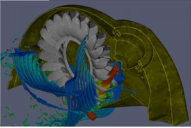
\includegraphics[width=0.3\textwidth]{10-11.png}~
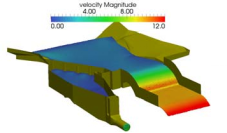
\includegraphics[width=0.3\textwidth]{10-12.png}~
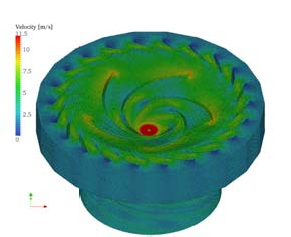
\includegraphics[width=0.3\textwidth]{10-13.png}
\caption{Left: free surface flows in an horizontal shaft Pelton casing. Center: free surface flows in a water intake. Right: confined transient flows during start-up of a simplified Francis turbine.}\label{fig:10}
\end{figure}

\end{abstract}


%%THE END OF ABSTRACT

\addbib

\end{document}
